\clearpage
\myparagraphold{Первый пример с \olly: a=1,2 и и=3,4}
\myindex{\olly}

Обе \FLD отработали:

\begin{figure}[H]
\centering
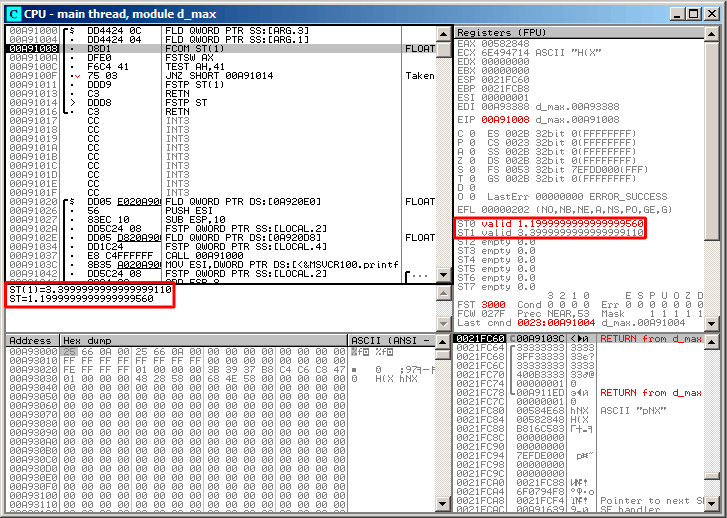
\includegraphics[scale=\FigScale]{patterns/12_FPU/3_comparison/x86/MSVC_Ox/olly1_1.png}
\caption{\olly: обе \FLD исполнились}
\label{fig:FPU_comparison_Ox_case1_olly1}
\end{figure}

Сейчас будет исполняться \FCOM: 
\olly показывает содержимое \ST{0} и \ST{1} для удобства.

\clearpage
\FCOM сработала:

\begin{figure}[H]
\centering
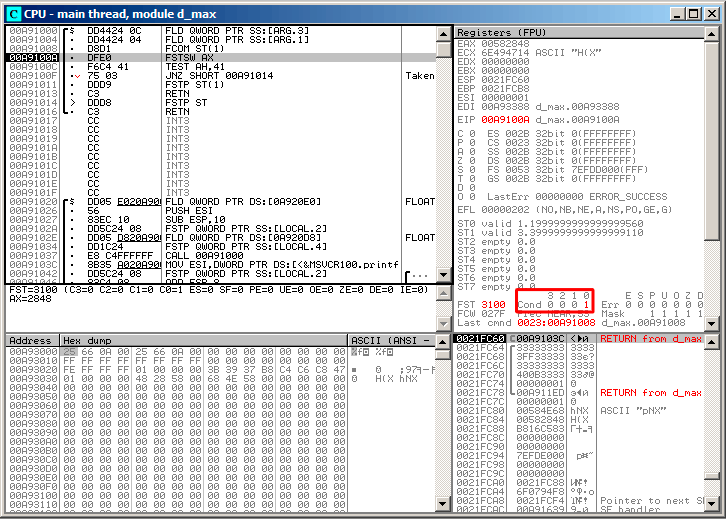
\includegraphics[scale=\FigScale]{patterns/12_FPU/3_comparison/x86/MSVC_Ox/olly1_2.png}
\caption{\olly: \FCOM исполнилась}
\label{fig:FPU_comparison_Ox_case1_olly2}
\end{figure}

\Czero установлен, остальные флаги сброшены.

\clearpage
\FNSTSW сработала, \GTT{AX}=0x3100:

\begin{figure}[H]
\centering
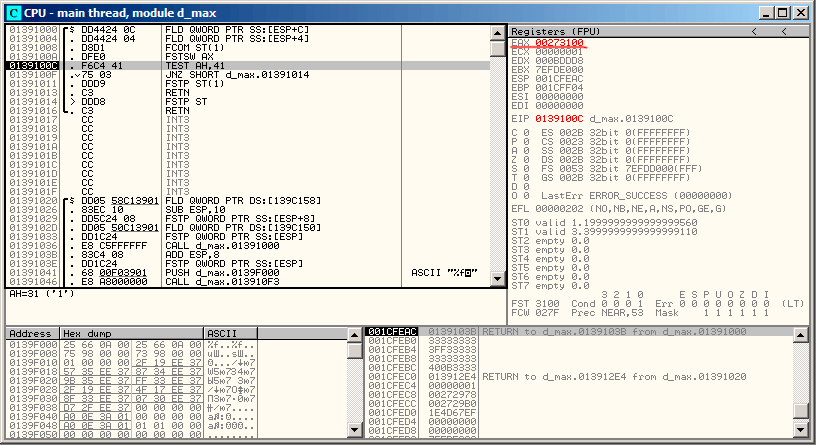
\includegraphics[scale=\FigScale]{patterns/12_FPU/3_comparison/x86/MSVC_Ox/olly1_3.png}
\caption{\olly: \FNSTSW исполнилась}
\label{fig:FPU_comparison_Ox_case1_olly3}
\end{figure}

\clearpage
\TEST сработала:

\begin{figure}[H]
\centering
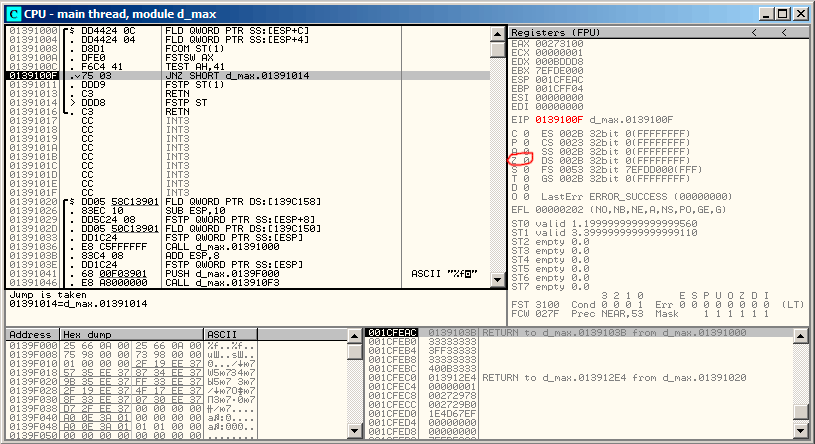
\includegraphics[scale=\FigScale]{patterns/12_FPU/3_comparison/x86/MSVC_Ox/olly1_4.png}
\caption{\olly: \TEST исполнилась}
\label{fig:FPU_comparison_Ox_case1_olly4}
\end{figure}

ZF=0, переход сейчас произойдет.

\clearpage
\INS{FSTP ST} (или \FSTP \ST{0}) сработала~--- 1,2 было вытолкнуто из стека, и на вершине осталось 3,4:

\begin{figure}[H]
\centering
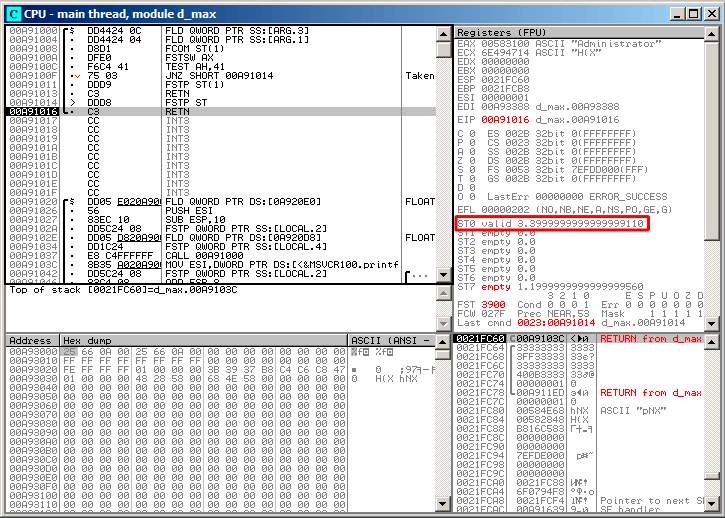
\includegraphics[scale=\FigScale]{patterns/12_FPU/3_comparison/x86/MSVC_Ox/olly1_5.png}
\caption{\olly: \FSTP исполнилась}
\label{fig:FPU_comparison_Ox_case1_olly5}
\end{figure}

Видно, что инструкция \INS{FSTP ST} работает просто как выталкивание одного значения из FPU-стека.

\clearpage
\myparagraphold{Второй пример с \olly: a=5,6 и b=-4}

Обе \FLD отработали:

\begin{figure}[H]
\centering
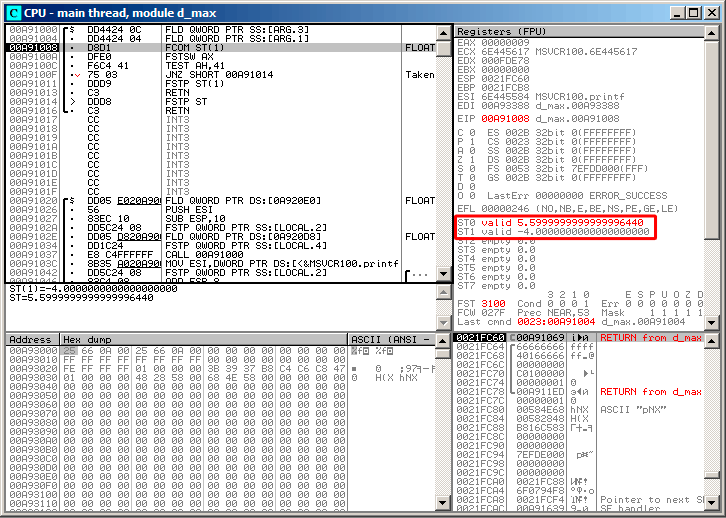
\includegraphics[scale=\FigScale]{patterns/12_FPU/3_comparison/x86/MSVC_Ox/olly2_1.png}
\caption{\olly: обе \FLD исполнились}
\label{fig:FPU_comparison_Ox_case2_olly1}
\end{figure}

Сейчас будет исполняться \FCOM.

\clearpage
\FCOM сработала:

\begin{figure}[H]
\centering
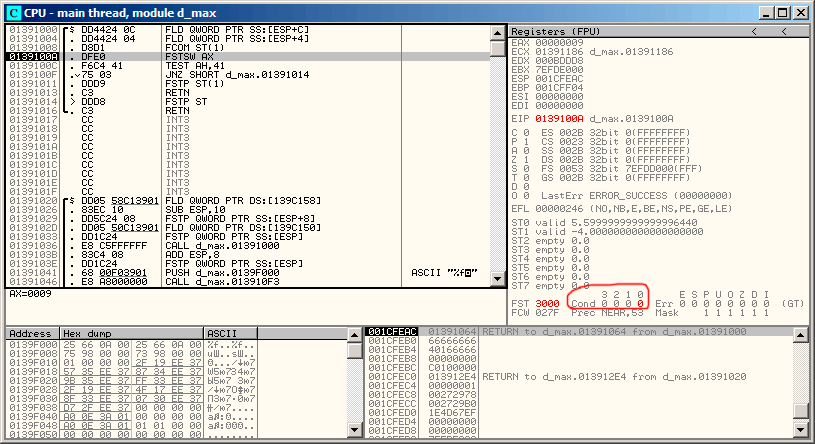
\includegraphics[scale=\FigScale]{patterns/12_FPU/3_comparison/x86/MSVC_Ox/olly2_2.png}
\caption{\olly: \FCOM исполнилась}
\label{fig:FPU_comparison_Ox_case2_olly2}
\end{figure}

Все condition-флаги сброшены.

\clearpage
\FNSTSW сработала, \GTT{AX}=0x3000:

\begin{figure}[H]
\centering
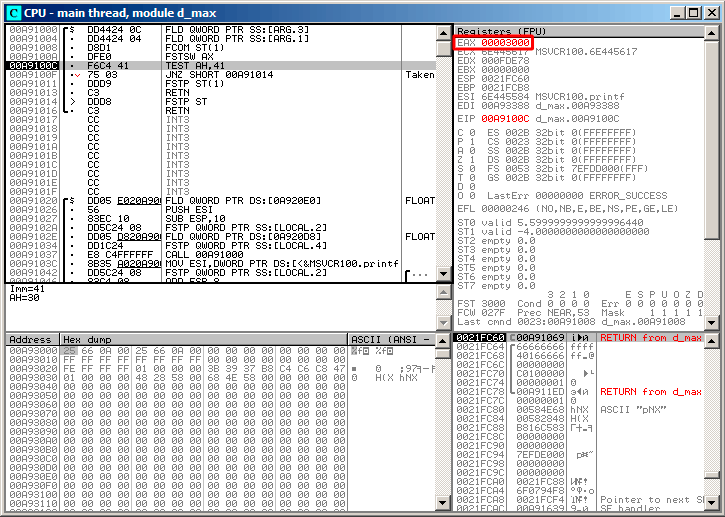
\includegraphics[scale=\FigScale]{patterns/12_FPU/3_comparison/x86/MSVC_Ox/olly2_3.png}
\caption{\olly: \FNSTSW исполнилась}
\label{fig:FPU_comparison_Ox_case2_olly3}
\end{figure}

\clearpage
\TEST сработала:

\begin{figure}[H]
\centering
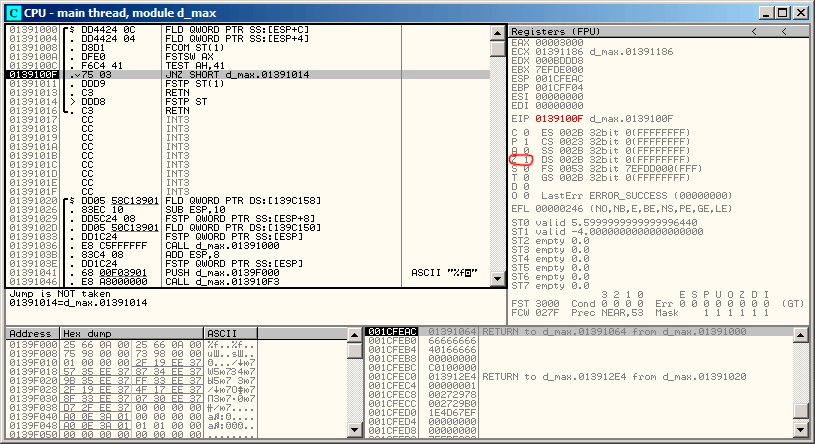
\includegraphics[scale=\FigScale]{patterns/12_FPU/3_comparison/x86/MSVC_Ox/olly2_4.png}
\caption{\olly: \TEST исполнилась}
\label{fig:FPU_comparison_Ox_case2_olly4}
\end{figure}

ZF=1, переход сейчас не произойдет.

\clearpage
\FSTP \ST{1} сработала: на вершине FPU-стека осталось значение 5,6.

\begin{figure}[H]
\centering
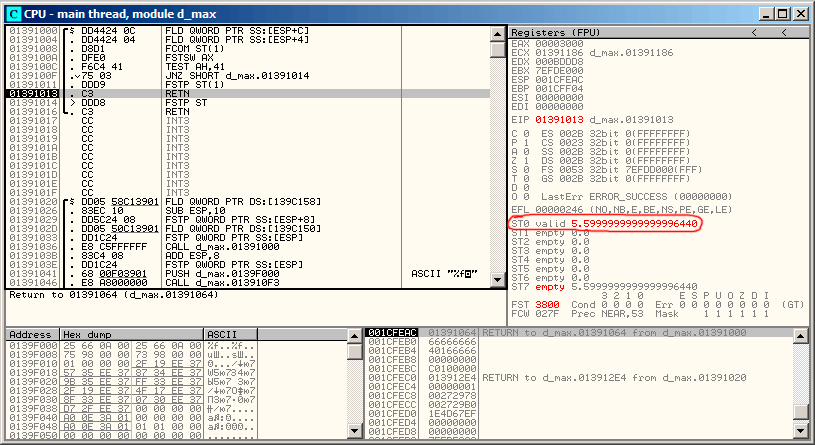
\includegraphics[scale=\FigScale]{patterns/12_FPU/3_comparison/x86/MSVC_Ox/olly2_5.png}
\caption{\olly: \FSTP исполнилась}
\label{fig:FPU_comparison_Ox_case2_olly5}
\end{figure}

Видно, что инструкция \FSTP \ST{1} работает так: оставляет значение на вершине стека, но обнуляет регистр \ST{1}.
